\chapter{ديناميكا الهيكل الخلوي وحركية الخلية}\label{ch:b3:cytoskeleton-motility}

عدلة تطارد بكتيريا عبر نسيج تزحف بعشرة
ميكرومترات في الدقيقة، وتغيّر اتجاهها في ثوانٍ حين تتبدل
الرائحة. وحويصلة ناقل عصبي مصنوعة في جسم عصبون
حركي تسافر مترًا نازلةً المحورَ إلى القدم، يجرّها بروتين
محرّك يخطو ثمانية نانومترات، مئة خطوة في الثانية،
أسبوعين. وأهداب بطانة القصبة الهوائية تضرب اثنتي عشرة مرة في الثانية في
أمواج منسّقة تحمل غبار يوم كامل مستنشقًا إلى البلعوم. وكل
هذا تؤديه ثلاثة أنواع من الخيوط البروتينية التي تتجمع و
تتفكك في ثوانٍ، ومحركات تحرق جزيء ATP واحدًا في كل
خطوة. والهيكل الخلوي ليس هيكلًا بمعنى الإطار
الثابت البتة؛ بل هو طقم من البوليمرات في دوران دائم، ودينامكيتها
\emph{هي} آلية الشكل والانقسام والحركة. ويتناول هذا الفصل
البوليمرات وحركيتها، والمحركات والفيزياء التي
تحدّها، وزحف الخلية، وضربة الأهداب و
الأسواط.

\section{ثلاثة بوليمرات}

\begin{definition}[خيوط الأكتين، والأنيبيبات الدقيقة، والخيوط المتوسطة]\label{def:b3:cytoskeleton-motility:filaments}
\index{خيط أكتين}\index{أنيبيب دقيق}\index{خيط متوسط}\index{القطبية!في الخيوط}\index{جسيم مركزي}
\emph{خيط الأكتين} بوليمر لولبي من طاقين من الأكتين
الكروي، ثخنه \qty{7}{nm}، وكل وحدة فيه \qty{2.7}{nm} على المحور،
وهو قطبي: إذ تنمو \emph{النهاية الشائكة} (الموجبة) أسرع من \emph{النهاية
المدببة} (السالبة)، وتحمل كل وحدة ATP يُحلمه بعد
الإدخال. و\emph{الأنيبيب الدقيق} أنبوب أجوف قطره الخارجي
\qty{25}{nm} مبني من ثلاثة عشر خيطًا أوليًا من ثنائيات التوبولين
$\alpha\beta$ (\qty{8}{nm} للثنائي)، وهو قطبي أيضًا، تنمو نهايته \emph{الموجبة}
أسرع وتكون نهايته \emph{السالبة} مثبتة عادةً عند
\emph{الجسيم المركزي} قرب النواة؛ وتحلمه الوحدة $\beta$
جزيء GTP فيها بعد الإدخال. و\emph{الخيط المتوسط} حبل
ثخنه \qty{10}{nm} مصنوع من بروتينات ملفوفة لولبيًا (كيراتينات في الظهارات،
وفيمنتين في المتوسطة، وخيوط عصبية في المحاور، ولامينات تحت
الغلاف النووي)، لا قطبية له، ولا نوكليوتيد، وهو أثبت بكثير ---
أي كبل يحمل الشد لا مسارًا ديناميكيًا. ويقع الأكتين في معظمه
تحت الغشاء الهيولي وفي البروزات؛ وتشعّ الأنيبيبات الدقيقة من
الجسيم المركزي وتعمل مسارات النقل بعيد المدى و
مغزلًا؛ وتمنح الخيوط المتوسطة الخليةَ ونواتها
مرونتهما الميكانيكية.
\end{definition}

\begin{omfigure}
\begin{tikzpicture}[every node/.style={font=\scriptsize}, >=stealth]
  % actin
  \begin{scope}
    \foreach \i in {0,...,11} { \fill[omThm!70] ({\i*0.4},{0.12*sin(\i*60)}) circle (0.17); }
    \node[below, align=center] at (2.2,-0.5) {خيط أكتين، \qty{7}{nm}\\لولب من طاقين، أكتين يحمل ATP\\الوحدة \qty{2.7}{nm} على المحور};
    \node[left] at (-0.3,0) {$-$ مدببة}; \node[right] at (4.6,0) {شائكة $+$};
  \end{scope}
  % microtubule
  \begin{scope}[xshift=7.2cm]
    \draw[thick, fill=omDef!25] (0,-0.55) rectangle (4.4,0.55);
    \foreach \y in {-0.35,-0.15,0.05,0.25} \draw[omDef] (0,\y) -- (4.4,\y);
    \foreach \x in {0.4,0.8,...,4.0} \draw[omDef] (\x,-0.55) -- (\x,0.55);
    \draw[thick] (4.4,0) ellipse (0.18 and 0.55); \draw[thick, fill=white] (4.4,0) ellipse (0.09 and 0.38);
    \node[below, align=center] at (2.2,-0.65) {أنيبيب دقيق، \qty{25}{nm}\\13 خيطًا أوليًا من التوبولين $\alpha\beta$ (GTP)\\طول الثنائي \qty{8}{nm}};
    \node[left] at (-0.2,0) {$-$}; \node[right] at (4.7,0) {$+$};
  \end{scope}
  % intermediate filament
  \begin{scope}[yshift=-2.9cm, xshift=3.6cm]
    \foreach \dd in {-0.12,0,0.12} \draw[omMeth!70!black, thick] plot[domain=0:4.4, samples=60] (\x, {\dd + 0.1*sin(\x*200 + \dd*400)});
    \node[below, align=center] at (2.2,-0.4) {خيط متوسط، \qty{10}{nm}\\حبل ملفوف لولبيًا (كيراتين، فيمنتين، لامين)، لا قطبية له ولا نوكليوتيد};
  \end{scope}
\end{tikzpicture}

{\small الخيوط الثلاثة بمقياس القطر. بوليمرات الأكتين والتوبولين
قطبية وتحلمه نوكليوتيدًا بعد التجمع، وهو ما
يجعلها ديناميكية؛ أما \omterm{def:b3:cytoskeleton-motility:filaments}{الخيط المتوسط} فحبل لا قطبية له
مبني للصبر.}
\end{omfigure}

\begin{omfigure}
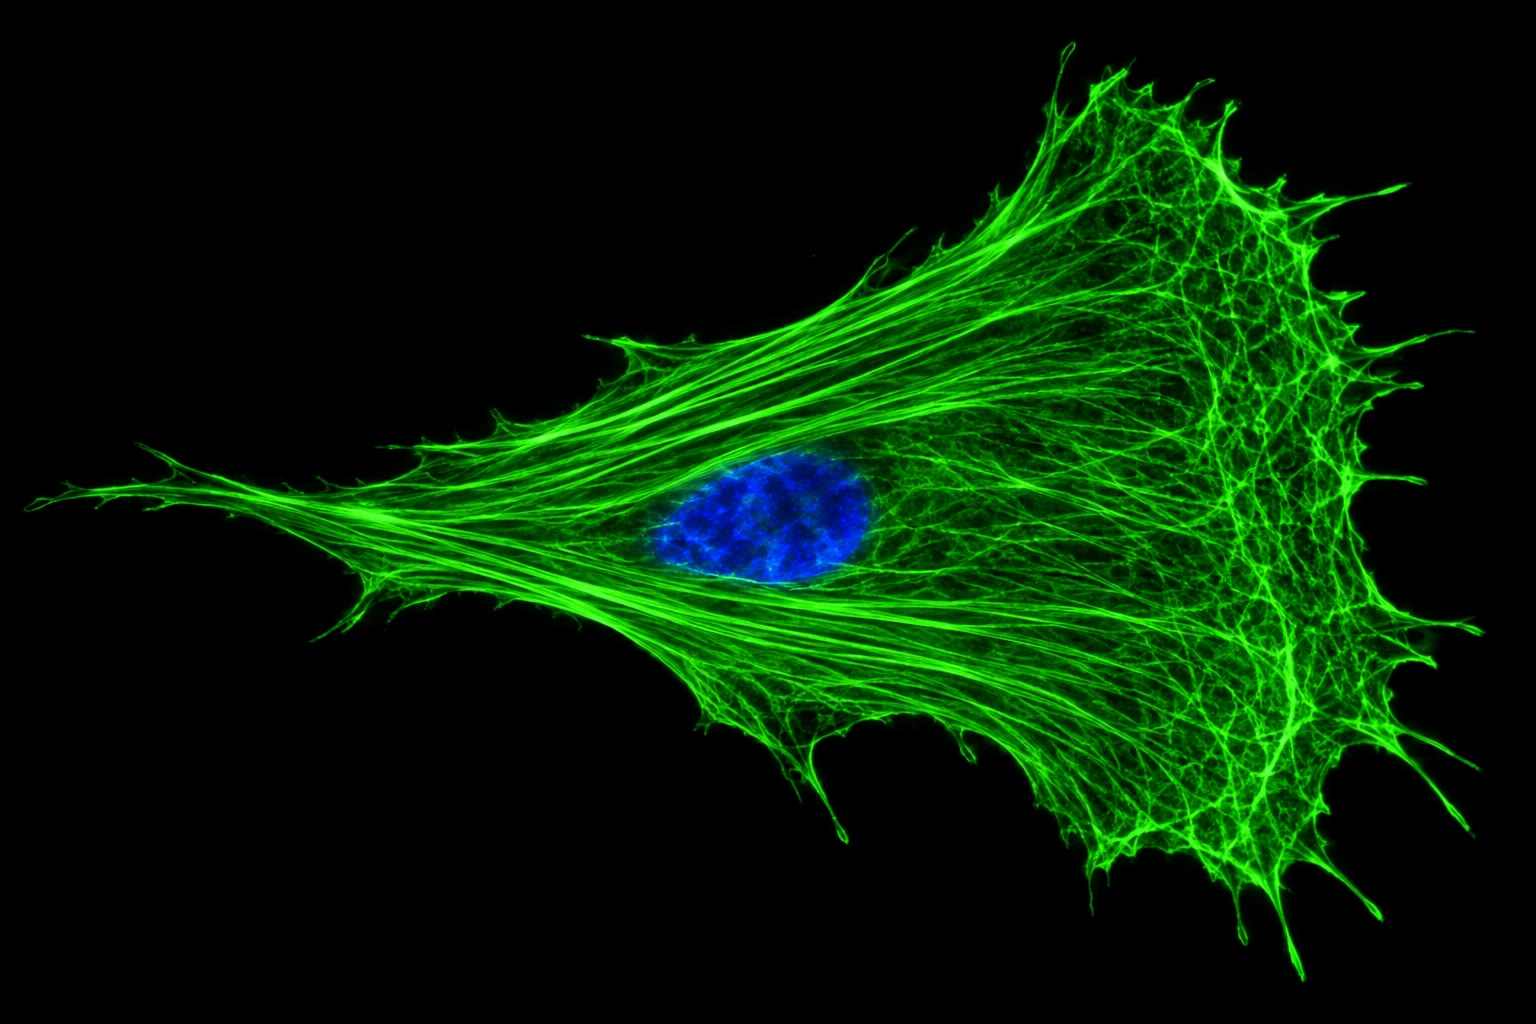
\includegraphics[width=0.54\linewidth]{images/book5/ai/b5-09-fibroblast-actin.jpg}\hspace{0.03\linewidth}
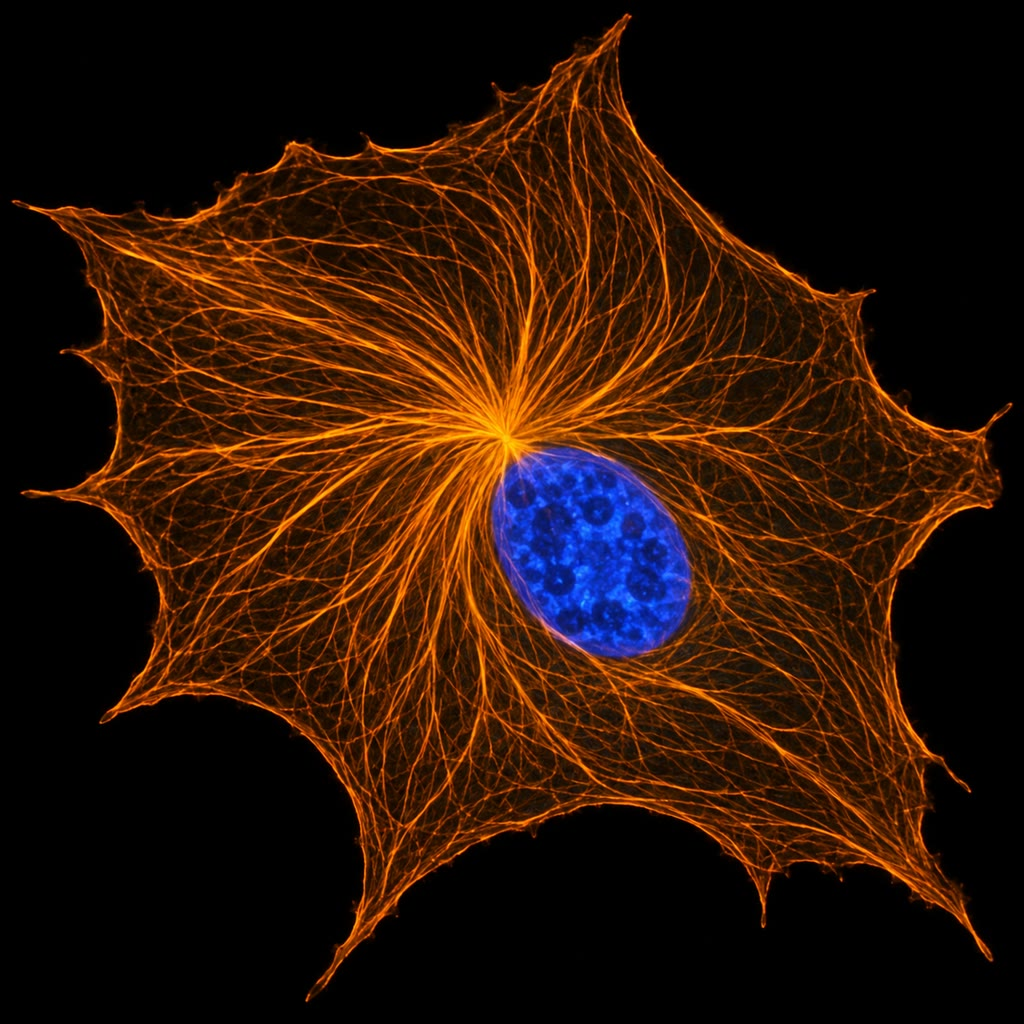
\includegraphics[width=0.36\linewidth]{images/book5/ai/b5-09-microtubules.jpg}

{\small يسارًا: الأكتين (بالأخضر) في خلية ليفية مهاجرة --- خيوط إجهاد
عبر الجسم، وشبكة كثيفة عند الحافة الأمامية العريضة على
اليمين. يمينًا: أنيبيبات دقيقة (بالبرتقالي) تشعّ من \omterm{def:b3:cytoskeleton-motility:filaments}{الجسيم المركزي}
بجوار النواة (بالأزرق) إلى حافة الخلية.}
\end{omfigure}

\section{حركية بوليمر}

\begin{theorem}[التركيز الحرج والدوران الشريطي]\label{thm:b3:cytoskeleton-motility:treadmilling}
\index{تركيز حرج}\index{دوران شريطي}
لتضف نهايةُ خيط وحداتٍ بمعدل $k_{\text{on}}C$، حيث
$C$ تركيز الوحيد الحر، ولتفقدها بمعدل
$k_{\text{off}}$. فتنمو النهاية إذا تجاوزت $C$ \emph{تركيزها
الحرج} $C_{c} = k_{\text{off}}/k_{\text{on}}$ وتتقلص دونه.
وإذا كان للنهايتين تركيزان حرجان مختلفان، $C_{c}^{+}
< C_{c}^{-}$، كان تركيز الوحيد عند الحالة المستقرة التي لا
يطول فيها الخيط ولا يقصر
\[
C_{\text{ss}} = \frac{k_{\text{off}}^{+} + k_{\text{off}}^{-}}
{k_{\text{on}}^{+} + k_{\text{on}}^{-}},
\qquad C_{c}^{+} < C_{\text{ss}} < C_{c}^{-},
\]
وتنمو النهاية الموجبة بينما تتقلص السالبة بالمعدل نفسه
$J = k_{\text{on}}^{+}C_{\text{ss}} - k_{\text{off}}^{+} > 0$: فتجري الوحدات
خلال الخيط من الموجبة إلى السالبة --- وهو \emph{\omterm{thm:b3:cytoskeleton-motility:treadmilling}{الدوران الشريطي}}
--- بكلفة نوكليوتيد واحد محلمَه لكل وحدة.
\end{theorem}
\begin{proof}
المعدل الصافي عند نهاية هو $k_{\text{on}}C - k_{\text{off}}$، وينعدم عند
$C_{c}$. وثبات الطول يقتضي انعدام مجموع المعدلين
الصافيين، وهو يعطي $C_{\text{ss}}$؛ وهي تقع بين التركيزين
الحرجين لأنها متوسط موزون لهما ($C_{\text{ss}} =
(k_{\text{on}}^{+}C_{c}^{+} + k_{\text{on}}^{-}C_{c}^{-})/(k_{\text{on}}^{+}
+ k_{\text{on}}^{-})$). وفوق $C_{c}^{+}$ تنمو النهاية الموجبة؛ ودون
$C_{c}^{-}$ تتقلص السالبة؛ والتدفق هو المعدل الصافي للنهاية الموجبة.
ونهايتا البوليمر الكيميائي الواحد كان ليكون لهما $C_{c}$ نفسه (أي
ثابت التوازن نفسه)، فالفرق يقتضي تغيّر الوحدة
بعد الإدخال --- أي حلمهة ATP أو GTP --- وهو ما
يجعل النهايتين تختلفان ويدفع ثمن الجريان.
\end{proof}

\begin{example}[الأكتين في أنبوب الاختبار]\label{ex:b3:cytoskeleton-motility:actin-numbers}
في الأكتين الحامل لجزيء ATP، $k_{\text{on}}^{+} = \qty{11.6}{\micro M^{-1}.s^{-1}}$،
و$k_{\text{off}}^{+} = \qty{1.4}{s^{-1}}$ ($C_{c}^{+} = \qty{0.12}{\micro
M}$)؛ و$k_{\text{on}}^{-} = \qty{1.3}{\micro M^{-1}.s^{-1}}$،
و$k_{\text{off}}^{-} = \qty{0.8}{s^{-1}}$ ($C_{c}^{-} = \qty{0.6}{\micro
M}$). ومنه $C_{\text{ss}} = 2.2/12.9 = \qty{0.17}{\micro M}$ و$J =
11.6\times 0.17 - 1.4 = 0.6$ وحدة في الثانية: أي \qty{1.6}{nm/s}،
وهو غير محسوس. أما في الخلية فتدور الخيوط أسرع مئة مرة،
لأن الكوفيلين يقطع ويجرد الأكتين القديم الحامل لجزيء ADP من
النهايات المدببة، ويحمّل البروفيلين أكتينًا طازجًا يحمل ATP على النهايات الشائكة، و
تقرر بروتينات الحجب أي النهايات الشائكة يُسمح لها بالنمو أصلًا: فالبوليمر
العاري يوفر الآلية، والمنظمات توفر السرعة.
\end{example}

\begin{omfigure}
\begin{tikzpicture}
\begin{axis}[
  width=0.7\linewidth, height=5.6cm,
  axis x line=bottom, axis y line=left,
  xmin=0, xmax=1.0, ymin=-1.6, ymax=4,
  xlabel={الأكتين الحر ($\unit{\micro M}$)}, ylabel={المعدل الصافي (وحدات/ثانية)},
  xlabel style={font=\small, at={(axis description cs:0.5,-0.12)}, anchor=north},
  ylabel style={font=\small},
  tick label style={font=\small}, xtick={0,0.2,0.4,0.6,0.8,1.0}, ytick={-1,0,1,2,3,4},
  clip=false,
]
\addplot[thin, gray, domain=0:1.0, samples=2] {0};
\addplot[very thick, omThm, domain=0:0.46, samples=2] {11.6*x-1.4};
\addplot[very thick, omDef, domain=0:1.0, samples=2] {1.3*x-0.8};
\draw[dashed, gray] (axis cs:0.17,-1.6) -- (axis cs:0.17,4);
\node[font=\scriptsize, omThm, anchor=south east] at (axis cs:0.44,3.1) {النهاية الشائكة};
\node[font=\scriptsize, omDef, anchor=north west] at (axis cs:0.62,-0.25) {النهاية المدببة};
\node[font=\scriptsize, anchor=south west] at (axis cs:0.19,3.5) {$C_{\text{ss}}$};
\fill[omThm] (axis cs:0.12,0) circle (2pt); \node[font=\scriptsize, anchor=north east] at (axis cs:0.11,-0.05) {$C_{c}^{+}$};
\fill[omDef] (axis cs:0.6,0) circle (2pt); \node[font=\scriptsize, anchor=south west] at (axis cs:0.61,0.05) {$C_{c}^{-}$};
\end{axis}
\end{tikzpicture}

{\small معدل النمو الصافي لكل نهاية من \omterm{def:b3:cytoskeleton-motility:filaments}{خيط أكتين} في مقابل الوحيد
الحر، بثوابت معدل المثال. فبين التركيزين
الحرجين تنمو النهاية الشائكة وتتقلص المدببة؛
وعند الخط المتقطع يلغي أحدهما الآخر تمامًا ويدور الخيط
دورانًا شريطيًا.}
\end{omfigure}

\begin{definition}[اللااستقرار الديناميكي]\label{def:b3:cytoskeleton-motility:instability}
\index{لااستقرار ديناميكي}\index{قلنسوة GTP}\index{كارثة}
تفعل الأنيبيبات الدقيقة شيئًا أغرب من \omterm{thm:b3:cytoskeleton-motility:treadmilling}{الدوران الشريطي}. فالنهاية الموجبة
النامية تحمل \emph{قلنسوة GTP} من ثنائيات مضافة حديثًا؛ وخلفها يُحلمه
GTP، ويبقى التوبولين الحامل لجزيء GDP، وهو يفضّل انتظامًا منحنيًا،
مشدودًا مستقيمًا في الشبيكة. فإذا فُقدت القلنسوة --- إذا
توقفت النهاية، أو بطؤ النمو --- انقشرت الخيوط الأولية المشدودة
خارجًا وقصر \omterm{def:b3:cytoskeleton-motility:filaments}{الأنيبيب الدقيق} بمعدل \qty{300}{nm/s}، أي عشرين ضعف
معدل نموه: وهي \emph{كارثة}، تنتهي حين يحطّ ثنائي
يحمل GTP وتتكوّن قلنسوة جديدة (أي \emph{إنقاذ}). ومن ثم ففي الجمهرة
الواحدة تنمو بعض الأنيبيبات بينما تنهار جاراتها: وهذا هو
\emph{اللااستقرار الديناميكي}. وهو يتيح للخلية أن تستكشف حجمها
بنهايات موجبة كل بضع دقائق وأن تعيد بناء المصفوفة كلها حين يتحرك
\omterm{def:b3:cytoskeleton-motility:filaments}{الجسيم المركزي} أو تنقسم الخلية. وتضبطه الخلية ببروتينات
تتعقب النهايات الموجبة، أو تثبّت (تاو، وMAP2)، أو تقطع (الكاتانين)
أو تزيل بلمرة الأنيبيبات (كينيزين-13)؛ ودواءا الكولشيسين
وقلويدات الونكا يحجبان التجمع والتاكسول يحجب التفكك، وكلها
سموم للمغزل الانقسامي تُستعمل ضد السرطان.
\end{definition}

\begin{proof}[شواهد]
راقب ميتشيسون وكيرشنر (1984) جمهرات من الأنيبيبات الدقيقة
النامية من جسيمات مركزية خارج الجسم. وبتمديد التوبولين دون
\omterm{thm:b3:cytoskeleton-motility:treadmilling}{التركيز الحرج}، توقعا أن تقصر الأنيبيبات كلها
ببطء؛ لكن عدد الأنيبيبات هبط بينما ظلت الناجية
تنمو --- فبعضها كان قد تفكك تمامًا وسريعًا، وبعضها لم يتفكك
البتة. ثم صُوّرت أنيبيبات مفردة لاحقًا بالمجهر الفيديوي فتبيّن أنها
تنتقل فجأةً بين أطوار نمو مطرد وتقلص سريع.
وفسّرت \omterm{def:b3:cytoskeleton-motility:instability}{قلنسوة GTP} الأمرين: فلا تنمو إلا النهايات المقلنسة، وفقدُ
القلنسوة حدث نادر من نمط الكل أو لا شيء.
\end{proof}

\section{المحركات}

\begin{definition}[البروتينات المحركة]\label{def:b3:cytoskeleton-motility:motors}
\index{ميوزين}\index{كينيزين}\index{داينين}\index{استمرارية}
\emph{البروتين المحرّك} يحوّل الطاقة الحرة لحلمهة ATP إلى
حركة موجَّهة على امتداد خيط: فمنها \emph{الميوزينات} على الأكتين (الميوزين
II، وهو محرّك العضلة والتقلص، نحو النهاية الشائكة؛ والميوزين V،
وهو حامل حويصلات ذو رأسين يخطو \qty{36}{nm})، و\emph{الكينيزينات}
على الأنيبيبات الدقيقة نحو النهاية الموجبة (فالكينيزين-1 يخطو \qty{8}{nm}،
أي ثنائي توبولين واحد، لكل ATP، يدًا فوق يد، بنحو \qty{800}{nm/s})،
و\emph{الداينينات} نحو النهاية السالبة (فالداينين الهيولي، مع
مهايئه الداينكتين، يجرّ الحمولة رجوعًا إلى مركز الخلية؛ وداينينات \omterm{def:b3:cytoskeleton-motility:cilia}{المحور الهدبي}
تثني الأهداب). ويكون المحرّك \emph{مستمرًا} إذا خطا خطوات كثيرة قبل أن
ينفصل: فالكينيزين-1 يمشي نحو ميكرومتر، أي مئة خطوة، وحده؛
أما رأس الميوزين II المفرد فيضرب ضربة واحدة ويطلق، فتحتاج العضلة إلى
مئات الرؤوس تعمل على خيط واحد. والمحركات تقرأ قطبية
المسار، فتكون جغرافيا الخلية --- نهايات موجبة عند المحيط، ونهايات
سالبة عند المركز --- خريطةً لأين يأخذ كل محرّك
حمولته.
\end{definition}

\begin{proof}[شواهد]
وجد فالي وريس وشيتز (1985) \omterm{def:b3:cytoskeleton-motility:motors}{الكينيزين} بروتينَ هيولى محور
الحبار الذي يجعل حبيبات لاتكس تنزلق على الأنيبيبات الدقيقة في الاتجاه
الموجب، وفُرزت في السنوات التالية البنية ذات الرأسين، واتجاه
كل أسرة، والشريك الراجع \omterm{def:b3:cytoskeleton-motility:motors}{الداينين}.
وأمسك سفوبودا وشميت وشناب وبلوك (1993) حبيبة تحمل
كينيزينًا واحدًا في مصيدة ضوئية وسجلوا موضعها بتمييز
نانومتري: فتقدمت الحبيبة بخطوات متقطعة قدرها
\qty{8}{nm}، خطوة لكل ATP عند تركيز ATP المنخفض، وتوقفت في مواجهة
قوة قدرها نحو \qty{6}{pN}. فرُئي السلّم الجزيئي
مباشرةً.
\end{proof}

\begin{omfigure}
\begin{tikzpicture}[every node/.style={font=\scriptsize}, >=stealth]
  % left: kinesin on a microtubule
  \begin{scope}
    \draw[thick, fill=omDef!25] (0,0) rectangle (5.4,0.5);
    \foreach \x in {0.4,0.8,...,5.2} \draw[omDef] (\x,0) -- (\x,0.5);
    \node[left] at (-0.1,0.25) {$-$}; \node[right] at (5.5,0.25) {$+$};
    % two heads, stalk, cargo
    \fill[omProp] (2.4,0.72) circle (0.2); \fill[omProp!60] (3.2,0.72) circle (0.2);
    \draw[thick, omProp!80!black] (2.6,0.85) -- (2.85,1.4) -- (3.05,0.85); \draw[thick, omProp!80!black] (2.85,1.4) -- (2.85,2.3);
    \draw[thick, fill=omExo!40] (2.85,2.7) circle (0.4); \node at (2.85,2.7) {حمولة};
    \draw[->, thick, omThm] (3.4,0.72) arc[start angle=180, end angle=0, radius=0.4] ; \node[right, omThm] at (3.85,1.15) {\qty{8}{nm} لكل ATP};
    \node[below, align=center] at (2.7,-0.1) {الكينيزين-1 يمشي يدًا فوق يد نحو النهاية الموجبة؛\\نحو $100$ خطوة في الثانية، \qty{0.8}{\micro m/s}};
  \end{scope}
  % right: optical trap staircase
  \begin{scope}[xshift=7.2cm, yshift=-0.6cm]
  \begin{axis}[
    width=5.6cm, height=4.4cm, axis lines=left,
    xmin=0, xmax=1.0, ymin=0, ymax=40,
    xlabel={الزمن (ثانية)}, ylabel={الموضع (nm)},
    xlabel style={font=\scriptsize, at={(axis description cs:0.5,-0.12)}, anchor=north},
    ylabel style={font=\scriptsize},
    tick label style={font=\scriptsize}, xtick={0,0.5,1.0}, ytick={0,8,16,24,32},
  ]
  \addplot[very thick, omProp!80!black, const plot] coordinates {(0,0) (0.18,8) (0.31,16) (0.55,24) (0.71,32) (1.0,32)};
  \end{axis}
  \node[font=\scriptsize, align=center] at (2.8,3.6) {محرّك واحد في مصيدة ضوئية،\\عند ATP منخفض: خطوات \qty{8}{nm}};
  \end{scope}
\end{tikzpicture}

{\small \omterm{def:b3:cytoskeleton-motility:motors}{الكينيزين} على مساره وأثره في مصيدة ضوئية. يتناوب
الرأسان، وكل خطوة تقدّم المحرّك بثنائي توبولين واحد،
أي \qty{8}{nm}؛ وعند ATP المنخفض تفصل بين الخطوات فترات انتظار للنوكليوتيد
التالي فيُرى السلّم مباشرةً.}
\end{omfigure}

\begin{proposition}[ما تسمح به الفيزياء لمحرّك]\label{prop:b3:cytoskeleton-motility:physics}
\index{قوة التوقف}\index{الطاقة الحرارية}\index{الانتشار في مقابل النقل}
تطلق حلمهة جزيء ATP واحد في الخلية نحو \qty{50}{kJ/mol}،
أي $8\times 10^{-20}$ جول للجزيء. والمحرّك الذي يتقدم $d$
لكل ATP في مواجهة قوة $F$ يبذل شغلًا $Fd$، فلا تستطيع \emph{قوة توقفه}
أن تتجاوز $F_{\max} = \Delta G/d$: فلخطوة \omterm{def:b3:cytoskeleton-motility:motors}{الكينيزين} البالغة \qty{8}{nm}،
تكون \qty{10}{pN}؛ والقيمة المقيسة \qty{6}{pN} تعني كفاءة قرب
\qty{60}{\%}، وهي أعلى من كفاءة أي محرّك. \omterm{prop:b3:cytoskeleton-motility:physics}{والطاقة الحرارية} $k_{B}T =
4.1\times 10^{-21}$ جول، أي \qty{4.1}{pN.nm}، ليست إلا عشرين جزءًا من
طاقة ATP لكنها تُسلَّم إلى المحرّك باستمرار ركلاتٍ
براونية؛ والمحرّك أداة تقوّمها، فتدع الرأس
ينتشر إلى الأمام ويرتبط حين يحطّ، فتُنفَق الطاقة الكيميائية
على جعل الخطوة غير عكوسة لا على الدفع.
والنقل بالمحرّك يغلب الانتشار على أي مسافة ذات شأن في
خلية كبيرة: فالحويصلة التي معامل انتشارها $D = \qty{1}{\micro
m^2/s}$ تحتاج زمنًا $L^{2}/2D$ لتجوب مسافة $L$ --- أي نصف
ثانية لميكرومتر، لكن \num{16000} سنة لمتر من محور ---
في حين يقطع محرّك سرعته \qty{1}{\micro m/s} المتر في اثني عشر يومًا.
\end{proposition}
\admitted

\section{كيف تزحف الخلية}

\begin{definition}[هجرة الخلية]\label{def:b3:cytoskeleton-motility:migration}
\index{صفيحة زائفة}\index{معقّد Arp2/3}\index{التصاق بؤري}\index{إنتغرين}\index{إنزيمات Rho من نمط GTPase}
تكرر الخلية الزاحفة دورة من أربع خطوات. \emph{البروز}: فعند
الحافة الأمامية يتبلمر الأكتين في مواجهة الغشاء صفيحةً، هي
\emph{الصفيحة الزائفة}، تبني شبكتَها المتفرعة
\emph{معقّد Arp2/3}، الذي ينوّي خيطًا جديدًا من جانب
خيط قائم بزاوية \qty{70}{\degree}، بينما يحدّ بروتين الحجب نمو كل
خيط ويعيد الكوفيلين تدوير الشبكة على بعد بضعة ميكرومترات
إلى الوراء؛ وتستكشف \emph{الأقدام الخيطية} الإصبعية من خيوط محزومة أمامها.
و\emph{الالتصاق}: يلتصق البروز الجديد بالركيزة عبر
\emph{الإنتغرينات}، وهي مستقبلات عابرة للغشاء تربط بروتينات الحشوة
في الخارج، وتربط الأكتين في الداخل عبر بروتينات مهايئة، متجمعة في
\emph{التصاقات بؤرية}. و\emph{التقلص}: يشد \omterm{def:b3:cytoskeleton-motility:motors}{الميوزين} II
خيوط الإجهاد المثبتة عند الالتصاقات، فيجرّ جسم الخلية
إلى الأمام. و\emph{الانكماش}: تنفكّ الالتصاقات في المؤخرة و
يُسحب الذيل إلى الداخل. وتنسّق الدورةَ ثلاثة إنزيمات GTPase صغيرة من
أسرة \emph{Rho} --- إذ يقود Rac الصفائح الزائفة، وCdc42 الأقدام الخيطية، و
Rho خيوط الإجهاد والتقلص --- وهي أهداف
المستقبلات التي تقرأ اتجاه تدرج كيميائي
(الانجذاب الكيميائي) أو صلابة الركيزة ونمطها.
\end{definition}

\begin{omfigure}
\begin{tikzpicture}[every node/.style={font=\scriptsize}, >=stealth]
  % substrate
  \draw[very thick, gray] (0,0) -- (12,0); \node[below right, gray] at (0,-0.05) {الركيزة (الحشوة)};
  % cell outline
  \draw[thick, omDef, fill=omDef!10] (1.0,0.05) .. controls (1.2,1.4) and (3.0,2.3) .. (5.0,2.2) .. controls (7.0,2.1) and (8.6,1.4) .. (9.8,0.6) .. controls (10.3,0.4) and (10.8,0.2) .. (11.2,0.05) -- cycle;
  % nucleus
  \draw[thick, fill=omDef!40] (4.6,1.1) ellipse (1.0 and 0.6); \node at (4.6,1.1) {النواة};
  % lamellipodium: branched actin
  \foreach \p/\a in {(9.9,0.3)/20,(10.1,0.5)/-10,(10.3,0.25)/35,(10.6,0.45)/5,(10.4,0.7)/-25,(9.7,0.7)/15} { \draw[omThm, thick] \p -- ++(\a:0.55); \draw[omThm, thick] \p ++(\a:0.3) -- ++(\a+70:0.35); }
  \node[right, align=left, omThm] at (11.3,1.3) {1. البروز:\\أكتين متفرع بمعقّد Arp2/3\\يدفع الغشاء};
  \draw[->, thick, omThm] (11.3,0.3) -- (11.9,0.3);
  % focal adhesions
  \foreach \x in {9.3,7.6,2.4} \fill[omProp] (\x-0.25,0.03) rectangle (\x+0.25,0.18);
  \node[below, omProp, align=center] at (9.3,-0.45) {2. الالتصاق: إنتغرينات،\\التصاقات بؤرية};
  % stress fibres and myosin
  \foreach \y in {0.45,0.75} \draw[omMeth!70!black, thick] (2.5,\y) -- (7.5,\y+0.1);
  \node[above, omMeth!70!black, align=center] at (7.8,2.3) {3. التقلص: الميوزين II\\على خيوط الإجهاد};
  \draw[->, thick, omMeth!70!black] (6.0,1.55) -- (6.8,1.55);
  % retraction at rear
  \draw[->, thick, gray] (0.8,0.9) -- (1.6,0.9); \node[above, align=center] at (1.4,2.35) {4. الانكماش:\\تنفكّ التصاقات المؤخرة};
\end{tikzpicture}

{\small دورة الزحف، واليسار إلى اليمين هو اتجاه
السير: بلمرة الأكتين المتفرع تدفع المقدمة إلى الخارج، وتثبّتها
الإنتغرينات، ويجرّ \omterm{def:b3:cytoskeleton-motility:motors}{الميوزين} الجسمَ إلى الأمام، وتطلق المؤخرة.}
\end{omfigure}

\begin{example}[مذنّب الليستيريا]\label{ex:b3:cytoskeleton-motility:listeria}
البكتيريا \emph{Listeria monocytogenes}، متى صارت داخل خلية،
تعرض على سطحها بروتينًا واحدًا هو ActA يستقدم
\omterm{def:b3:cytoskeleton-motility:migration}{معقّد Arp2/3} عند المضيف. فيتبلمر الأكتين عند سطح البكتيريا و
يُترك خلفها ذيلًا؛ وتُدفع البكتيريا عبر الهيولى
بما يصل إلى \qty{0.5}{\micro m/s} وإلى الخلايا المجاورة من غير أن تغادر
العصارة قط. والذيل \omterm{def:b3:cytoskeleton-motility:migration}{صفيحة زائفة} مقلوبة، ببروتين
واحد حيث تستعمل الخلية عشرات، وقد بيّن أن بلمرة
الأكتين وحدها --- بلا أي محرّك --- تولّد قوة
البروز: فكل وحدة تندس بين الشبكة والغشاء،
حين يفتح تقلب حراري ثغرة، تقدّم المقدمة
بمقدار \qty{2.7}{nm}.
\end{example}

\begin{method}[مراقبة دوران البوليمرات]\label{met:b3:cytoskeleton-motility:frap}
\index{استعادة التألق بعد التبييض}\index{مجهرية البقع}
لقياس ديناميكا منظومة خيوط في خلية حية: (1)
عبّر عن الوحدة ملحومةً ببروتين متألق بمستوى منخفض، حتى
تُدمج في البوليمر الأصلي؛ (2) إما أن تبيّض
منطقة صغيرة بنبضة ليزر شديدة وتصوّر عودة
التألق مع تبادل الوحدات غير المبيَّضة إلى الداخل (\emph{\omterm{met:b3:cytoskeleton-motility:frap}{استعادة
التألق بعد التبييض}}، FRAP) --- وزمن النصف هو
زمن مكث الوحدات، والنسبة التي لا تعود أبدًا هي
المخزون الساكن؛ أو (3) عبّر عن قدر ضئيل من الوحدة الموسومة حتى يبدو
البوليمر \emph{بقعًا} متناثرة، وتعقبها: فحركتها
هي جريان \omterm{thm:b3:cytoskeleton-motility:treadmilling}{الدوران الشريطي}، وظهورها واختفاؤها
هما التجمع والتفكك. وفي \omterm{def:b3:cytoskeleton-motility:migration}{الصفيحة الزائفة} تجري البقع
إلى الوراء بميكرومتر في الدقيقة نسبةً إلى الركيزة بينما تتقدم
الحافة: فالشبكة تُبنى في المقدمة وتُستهلك على بعد بضعة
ميكرومترات خلفها.
\end{method}

\section{الأهداب والأسواط ومحرّك دوّار}

\begin{definition}[الأهداب والأسواط]\label{def:b3:cytoskeleton-motility:cilia}
\index{هدب}\index{محور هدبي}\index{داينين محوري}\index{هدب أولي}\index{نقل داخل سوطي}
\emph{الهدب} أو \emph{السوط} في حقيقيات النوى امتداد مغطى
بغشاء مبني على \emph{المحور الهدبي}: أي تسعة أنيبيبات مزدوجة في
حلقة حول زوج مركزي، تمسكها وصلات النكسين والأشواك الشعاعية، و
تنمو من جسم قاعدي، وهو مريكز معدَّل. و\emph{الداينينات المحورية}
الملتصقة بكل مزدوج تمشي على المزدوج المجاور نحو نهايته
السالبة عند القاعدة؛ ولأن المزدوجات مربوطة بعضها ببعض فهي لا تستطيع
الانزلاق بحرية، فيتحوّل الانزلاق إلى انثناء، ينتشر
على امتداد المحور موجةً بتبديل الداينينات الفاعلة من جانب
من الحلقة إلى الآخر. وطول الهدب \qtyrange{5}{10}{\micro m}
ويضرب \numrange{10}{20} مرة في الثانية؛ أما سوط النطفة فطوله
\qty{50}{\micro m} ويتموج. وتُحمل بروتينات الهدب
صعودًا من جسم الخلية بالكينيزين-2 ورجوعًا بالداينين-2 على امتداد
المزدوجات، وهو \emph{النقل داخل السوطي}، وهو أيضًا كيفية بناء
\emph{الهدب الأولي} غير المحرّك --- الموجود، واحدًا في كل خلية، على معظم
خلايا الفقاريات --- وذلك الهدب هوائي حسي،
يؤوي مستقبلات للضوء (القطعة الخارجية للعصية)، وللروائح، وللجريان و
لإشارات التطور، وتسبب عيوبه \emph{اعتلالات الأهداب}:
الكلى متعددة الكيسات، وتنكس الشبكية، والبدانة، وأصابع زائدة.
\end{definition}

\begin{omfigure}
\begin{tikzpicture}[every node/.style={font=\scriptsize}, >=stealth]
  % axoneme cross-section
  \begin{scope}
    \draw[thick, omDef!60] (0,0) circle (1.75);
    \foreach \i in {0,...,8} { \begin{scope}[rotate=\i*40] \draw[thick, fill=omDef!30] (0,1.3) circle (0.16); \draw[thick, fill=omDef!30] (0.27,1.22) circle (0.13); \draw[omProp, thick] (0.15,1.05) -- (0.05,0.5); \draw[omThm, thick] (0.4,1.28) -- (0.62,1.2); \end{scope} }
    \draw[thick, fill=omDef!30] (-0.15,0) circle (0.16); \draw[thick, fill=omDef!30] (0.15,0) circle (0.16);
    \node[right, align=left] at (2.0,1.2) {9 أنيبيبات مزدوجة}; \draw (1.9,1.2) -- (1.35,1.0);
    \node[right, align=left] at (2.0,0.4) {الزوج المركزي}; \draw (1.9,0.4) -- (0.35,0.1);
    \node[right, align=left, omThm] at (2.0,-0.4) {أذرع الداينين على كل\\مزدوج تبلغ التالي}; \draw[omThm] (1.9,-0.3) -- (1.0,-0.85);
    \node[right, align=left, omProp] at (2.0,-1.3) {أشواك شعاعية}; \draw[omProp] (1.9,-1.3) -- (0.4,-0.7);
    \node[below] at (0,-1.9) {المحور الهدبي، قطره \qty{0.25}{\micro m}};
  \end{scope}
  % bending from sliding
  \begin{scope}[xshift=7.6cm]
    \draw[very thick, omDef] (0,-1.6) -- (0,1.6); \draw[very thick, omDef] (0.5,-1.6) -- (0.5,1.6);
    \draw[->, thick, omThm] (0.1,0.5) -- (0.4,0.5); \draw[->, thick, omThm] (0.1,-0.2) -- (0.4,-0.2);
    \node[below, align=center] at (0.25,-1.7) {داينينات على مزدوج\\تدفع الجار\\نحو القمة};
    \draw[->, thick] (1.5,0) -- (2.5,0);
    \draw[very thick, omDef] (3.6,-1.6) .. controls (3.6,-0.3) and (4.6,0.5) .. (4.4,1.6); \draw[very thick, omDef] (4.1,-1.6) .. controls (4.1,-0.3) and (5.1,0.5) .. (4.9,1.6);
    \node[below, align=center] at (4.3,-1.7) {مربوطة عند القاعدة وبالنكسين،\\فلا تستطيع المزدوجات الانزلاق:\\فتنثني};
  \end{scope}
\end{tikzpicture}

{\small \omterm{def:b3:cytoskeleton-motility:cilia}{المحور الهدبي} في مقطع عرضي (يسارًا): تسعة مزدوجات حول
زوج مركزي، مع أذرع \omterm{def:b3:cytoskeleton-motility:motors}{الداينين} والأشواك الشعاعية. يمينًا: تزلق الداينينات
مزدوجًا على التالي، ولأن المزدوجات مربوطة يصير
الانزلاق انثناءً يسري على امتداد \omterm{def:b3:cytoskeleton-motility:cilia}{الهدب}.}
\end{omfigure}

\begin{omfigure}
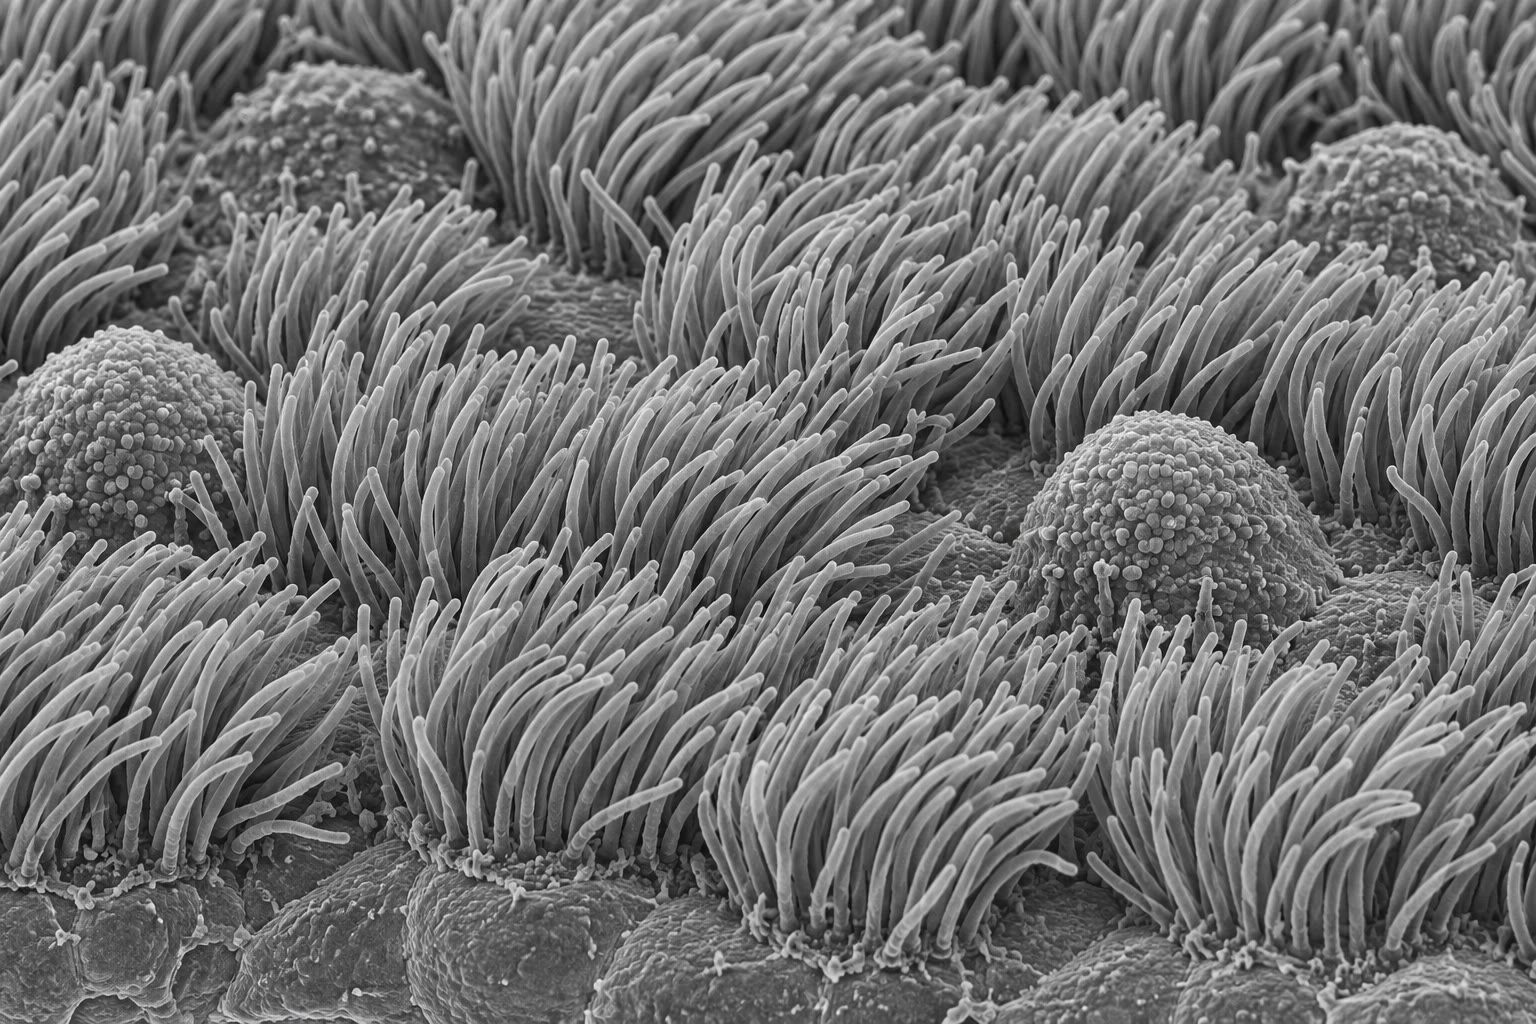
\includegraphics[width=0.54\linewidth]{images/book5/ai/b5-09-cilia-sem.jpg}\hspace{0.03\linewidth}
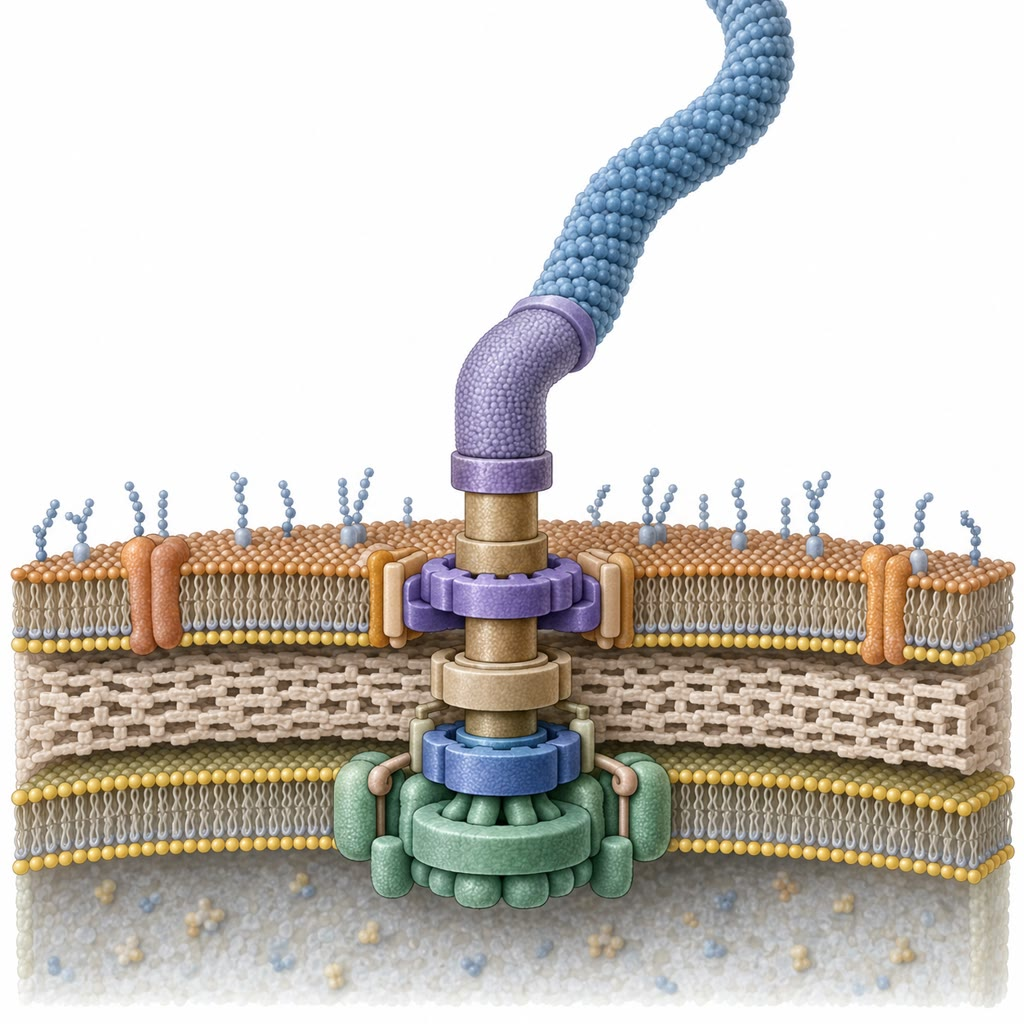
\includegraphics[width=0.36\linewidth]{images/book5/ai/b5-09-flagellar-motor.jpg}

{\small يسارًا: ظهارة القصبة الهوائية المهدبة في المجهر الإلكتروني
الماسح، بساط من الأهداب بين خلايا قبّية تفرز
المخاط. يمينًا: \omterm{prop:b3:cytoskeleton-motility:flagellar-motor}{محرّك السوط البكتيري}، وهو مكنة دوّارة من حلقات
في غلاف الخلية يقودها جريان البروتونات.}
\end{omfigure}

\begin{proposition}[محرّك السوط البكتيري]\label{prop:b3:cytoskeleton-motility:flagellar-motor}
\index{محرّك سوطي}\index{الجري والتخبط}
السوط البكتيري لا صلة له بالسوط في حقيقيات النوى: فهو خيط
لولبي صلب من الفلاجيلين، ثخنه \qty{20}{nm} وطوله عدة
ميكرومترات، يديره \emph{محرّك دوّار} مغروس في غلاف
الخلية --- أي دوّار من نحو خمسة وأربعين بروتينًا تحيط به حلقة
من وحدات ثابتة، كل منها قناة تجري فيها البروتونات هابطةً
تدرجها إلى داخل الخلية، بنحو ألف بروتون في الدورة.
ويدور المحرّك بما يصل إلى \qty{300}{Hz}، وينعكس اتجاهه في
مليثانية، ويولّد عزمًا قدره نحو \qty{1000}{pN.nm}؛ وهو
مبني من نحو عشرين بروتينًا تُفتح مورّثاتها بالترتيب
الذي تُجمَّع به الأجزاء، من الداخل إلى الخارج. وفي \emph{E.~coli}،
يحزم الدوران عكس عقارب الساعة الأسواط المتعددة في
مروحة \emph{فتجري} الخلية مستقيمةً؛ والتبديل إلى اتجاه عقارب الساعة
يبعثر الحزمة \emph{فتتخبط} الخلية إلى اتجاه عشوائي جديد.
ولا يحيّز مسلك الانجذاب الكيميائي إلا تواتر
التخبطات --- فيقلّ حين تتحسن الأحوال --- ويكفي ذلك
لتسلّق تدرج.
\end{proposition}

\begin{remark}[الهيكل الخلوي فعل لا اسم]\label{rem:b3:cytoskeleton-motility:verb}
لا يكاد شيء مما وُصف في هذا الفصل يكون بنيةً بالمعنى
الذي يكون به العظم بنيةً: \omterm{def:b3:cytoskeleton-motility:migration}{فالصفيحة الزائفة} موجة بلمرة، و
مغزل \cref{ch:b3:cell-cycle-apoptosis} حالة مستقرة من أنيبيبات نامية
ومنهارة، وضربة \omterm{def:b3:cytoskeleton-motility:cilia}{الهدب} نمط تبديل
للمحركات. والدوران ليس كلفة تحتملها الخلية بل الآلية
نفسها، ولهذا تعمل كل واحدة من هذه المنظومات على حلمهة
النوكليوتيد وتتوقف في دقائق من نفاد ATP، ولهذا تكون
السموم التي تجمّد البوليمرات في أي من الحالتين --- التاكسول أو
الكولشيسين، والفالويدين أو السيتوكالازين --- مميتة سواء بسواء.
\end{remark}

\section{تمارين}

\begin{exercise}[$\star$]\label{exo:b3:cytoskeleton-motility:1}
قارن بين خيوط الأكتين والأنيبيبات الدقيقة والخيوط المتوسطة في
القطر والوحدة والقطبية والنوكليوتيد والدور النمطي.
\end{exercise}

\begin{exercise}[$\star$]\label{exo:b3:cytoskeleton-motility:2}
عرّف \omterm{thm:b3:cytoskeleton-motility:treadmilling}{التركيز الحرج}. ولماذا يكون لنهايتي \omterm{def:b3:cytoskeleton-motility:filaments}{خيط الأكتين}
تركيزان حرجان مختلفان، وماذا كان ليحدث لو
تساويا؟
\end{exercise}

\begin{exercise}[$\star$]\label{exo:b3:cytoskeleton-motility:3}
سمِّ محرّكًا لكل مما يلي: حويصلة نحو محيط الخلية على
الأنيبيبات الدقيقة؛ وحويصلة نحو المركز؛ وتقلص خيط
إجهاد؛ وانثناء \omterm{def:b3:cytoskeleton-motility:cilia}{هدب}. وأعطِ الاتجاه الذي يسلكه كل منها على مساره.
\end{exercise}

\begin{exercise}[$\star$]\label{exo:b3:cytoskeleton-motility:4}
عدّد خطوات دورة الزحف الأربع وإنزيم GTPase من أسرة Rho
الذي يحكم كلًا من الثلاث الأولى.
\end{exercise}

\begin{exercise}[$\star\star$]\label{exo:b3:cytoskeleton-motility:5}
نهاية بوليمر موجبة لها $k_{\text{on}} = \qty{5}{\micro M^{-1}.s^{-1}}$
و$k_{\text{off}} = \qty{1}{s^{-1}}$، ونهايته السالبة $k_{\text{on}} =
\qty{1}{\micro M^{-1}.s^{-1}}$ و$k_{\text{off}} = \qty{0.8}{s^{-1}}$.
أوجد التركيزين الحرجين، وتركيز الحالة المستقرة
ومعدل \omterm{thm:b3:cytoskeleton-motility:treadmilling}{الدوران الشريطي} بالوحدات في الثانية، ومن أجل
وحدات قدرها \qty{2.7}{nm}، بالنانومترات في الثانية.
\end{exercise}

\begin{exercise}[$\star\star$]\label{exo:b3:cytoskeleton-motility:6}
يمشي \omterm{def:b3:cytoskeleton-motility:motors}{الكينيزين} بسرعة \qty{800}{nm/s} بخطوات \qty{8}{nm}، لكل منها ATP واحد.
فكم ATP في الثانية لكل محرّك؟ ومحور العصبون طوله \qty{1}{m}: فكم
تستغرق الرحلة، وكم ATP ينفق محرّك واحد فيها؟ قارن
بزمن الانتشار من \cref{prop:b3:cytoskeleton-motility:physics}.
\end{exercise}

\begin{exercise}[$\star\star$]\label{exo:b3:cytoskeleton-motility:7}
يخطو \omterm{def:b3:cytoskeleton-motility:motors}{الميوزين} V \qty{36}{nm} لكل ATP. فما قوة توقفه القصوى،
ولماذا تكون أقل من قوة \omterm{def:b3:cytoskeleton-motility:motors}{الكينيزين}؟ وأي المحركين أنسب
لحمل حمولة كبيرة، وأيهما للحركة السريعة؟
\end{exercise}

\begin{exercise}[$\star\star$]\label{exo:b3:cytoskeleton-motility:8}
تنبأ بالأثر في خلية منقسمة، وفي خلية زاحفة، لكل من (أ)
التاكسول، و(ب) الكولشيسين، و(ج) السيتوكالازين، و(د) مثبط Rac، و
فسّر كل أثر من الآلية.
\end{exercise}

\begin{exercise}[$\star\star$]\label{exo:b3:cytoskeleton-motility:9}
في تجربة FRAP على \omterm{def:b3:cytoskeleton-motility:migration}{صفيحة زائفة}، يعود التألق بزمن
نصف قدره \qty{20}{s} إلى \qty{90}{\%} من قيمته الابتدائية. فما
زمن مكث الأكتين في الشبكة وما النسبة الساكنة؟
وتجري البقع إلى الوراء بسرعة \qty{1.5}{\micro m/min} بينما تتقدم الحافة
بسرعة \qty{1}{\micro m/min}: فبأي معدل يتبلمر الأكتين
عند الحافة؟
\end{exercise}

\begin{exercise}[$\star\star\star$]\label{exo:b3:cytoskeleton-motility:10}
فسّر \omterm{def:b3:cytoskeleton-motility:instability}{اللااستقرار الديناميكي} بدلالة \omterm{def:b3:cytoskeleton-motility:instability}{قلنسوة GTP}، وبيّن لماذا
تصير جمهرةُ أنيبيبات دقيقة مبقاة فوق \omterm{thm:b3:cytoskeleton-motility:treadmilling}{التركيز الحرج} بقليل
ثنائية النمط في الطول لا منتظمة. وما الذي تكسبه الخلية
من سلوك يبدد GTP؟
\end{exercise}

\begin{exercise}[$\star\star\star$]\label{exo:b3:cytoskeleton-motility:11}
بكتيريا طولها \qty{2}{\micro m} تسبح بسرعة \qty{25}{\micro m/s}. وفي
الماء عند هذا المقياس تهيمن المقاومة اللزجة وتتوقف الخلية في
نانومتر حين يتوقف المحرّك. فسّر لماذا لا تستطيع الحركة الترادفية
(المجداف) أن تدفعها ويستطيع لولب دوّار ذلك، وقدّر
عدد البروتونات التي ينفقها المحرّك في الثانية عند \qty{100}{Hz}.
\end{exercise}

\begin{exercise}[$\star\star\star$]\label{exo:b3:cytoskeleton-motility:12}
متلازمة كارتاجينر --- أهداب لا تتحرك --- تعطي التهاب قصبات مزمنًا،
وعقمًا عند الذكور، وقلبًا على الجانب الأيمن عند نصف المرضى.
فسّر كلًا منها من بيولوجيا \omterm{def:b3:cytoskeleton-motility:cilia}{المحور الهدبي}، وقل لماذا لا يصيب الأخير
إلا النصف.
\end{exercise}

\section{مسألة: عدلة تتحرك}

\begin{problem}[{مسألة نهاية الأسبوع --- ميزانية الأكتين في عدلة
معدودةً، ودورانها الشريطي محسوبًا، ورحلة حويصلة في محور
موقوتةً في مواجهة الانتشار، وكفاءة محرّك مقيسة، و
بلمرة جبهة الزحف وكلفتها من ATP محسوبتين، وتنتهي إلى
معدل الدوران الشريطي، وزمن عبور المحور، وATP الذي تحرقه
صفيحة زائفة في الثانية}]
\label{pb:b3:cytoskeleton-motility:1}
معطيات: عدلة حجمها \qty{300}{\micro m^3} تحوي أكتينًا بتركيز
\qty{200}{\micro M}، نصفه متبلمر؛ والوحدة تضيف \qty{2.7}{nm} إلى
الخيط. وثوابت معدل الأكتين كما في
\cref{ex:b3:cytoskeleton-motility:actin-numbers}. \omterm{def:b3:cytoskeleton-motility:motors}{والكينيزين}: خطوات \qty{8}{nm}،
وسرعة \qty{800}{nm/s}، وقوة توقف \qty{6}{pN}؛ وحلمهة ATP
$\Delta G = \qty{50}{kJ/mol}$؛ و$k_{B}T = \qty{4.1}{pN.nm}$؛ ومعامل
انتشار الحويصلة \qty{1}{\micro m^2/s}؛ وطول المحور \qty{1}{m}. و
\omterm{def:b3:cytoskeleton-motility:migration}{الصفيحة الزائفة} عرضها \qty{20}{\micro m} وفيها $200$ خيط لكل
ميكرومتر من الحافة، وتتقدم بسرعة \qty{10}{\micro m/min}؛ وتُفكَّك الشبكة
على بعد \qty{3}{\micro m} خلف الحافة.

\medskip
\noindent\textbf{الجزء الأول --- ميزانية الأكتين.}
\begin{enumerate}
  \item كم جزيء أكتين تحوي الخلية، وكم منها
        في خيوط؟
  \item ما الطول الكلي للخيوط الذي يعادل ذلك؟ وإذا كان متوسط الخيط
        \qty{0.25}{\micro m}، فكم خيطًا؟
  \item الأكتين الحر \qty{100}{\micro M}، أي فوق \omterm{thm:b3:cytoskeleton-motility:treadmilling}{التركيز الحرج}
        للنهاية الشائكة بكثير. فلماذا لا تنمو الخيوط ببساطة
        حتى ينفد الوحيد؟ (بروتينان.)
  \item \omterm{thm:b3:cytoskeleton-motility:treadmilling}{الدوران الشريطي} خارج الجسم: احسب $C_{\text{ss}}$ و$J$ من
        ثوابت المعدل، وسرعة \omterm{thm:b3:cytoskeleton-motility:treadmilling}{الدوران الشريطي} بالنانومترات في
        الثانية وبالميكرومترات في الدقيقة.
  \item وفي الخلية تبلغ السرعة الفعلية \qty{1}{\micro m/min}. فبأي
        عامل تسرّع المنظماتُ البوليمرَ العاري؟
  \item كل وحدة تدور شريطيًا تكلّف ATP واحدًا. فإذا دارت الخيوط البالغة $2\times 10^{5}$
        كلها بالسرعة الخلوية، فكم ATP في
        الثانية، وما نسبة ذلك من دوران الخلية الكلي البالغ
        نحو $10^{9}$ ATP في الثانية؟
\end{enumerate}

\medskip
\noindent\textbf{الجزء الثاني --- حويصلة تنزل المحور.}
\begin{enumerate}[resume]
  \item كم تستغرق حويصلة يقودها \omterm{def:b3:cytoskeleton-motility:motors}{كينيزين} لتقطع المحور،
        وكم خطوة وكم ATP ينفق المحرّك؟
  \item وكم يستغرق الانتشار على مدى \qty{1}{m}؟ وعلى مدى
        \qty{10}{\micro m}، وهو عرض جسم خلية؟ وماذا تقول
        المقارنة عن أين تستطيع الخلايا أن تعتمد على
        الانتشار؟
  \item احسب الطاقة لكل ATP بالجول وبوحدات $k_{B}T$.
  \item القوة القصوى لمحرّك خطواته \qty{8}{nm}، و
        كفاءة \omterm{def:b3:cytoskeleton-motility:motors}{الكينيزين} عند التوقف.
  \item حويصلة نصف قطرها \qty{100}{nm} في هيولى لزوجتها
        \qty{0.01}{Pa.s} (أي عشرة أضعاف الماء) تتحرك بسرعة \qty{800}{nm/s}
        تشعر بمقاومة $F = 6\pi\eta r v$. احسبها، وقارنها \omterm{prop:b3:cytoskeleton-motility:physics}{بقوة
        التوقف}: كم محرّكًا يلزم؟
  \item يحمل محور العصبون نحو $10^{4}$ حويصلة في وقت واحد. فما
        استهلاك النقل الكلي من ATP في الثانية، وكيف
        يقارن بكلفة إطلاق العصبون البالغة نحو
        $10^{9}$ ATP في الثانية؟ وماذا يعني ذلك لعصبون
        تخفق متقدراته؟
\end{enumerate}

\medskip
\noindent\textbf{الجزء الثالث --- الجبهة.}
\begin{enumerate}[resume]
  \item حوّل سرعة الحافة إلى نانومترات في الثانية، واحسب
        عدد الوحدات في الثانية التي يجب أن يضيفها كل خيط ليواكب
        ذلك.
  \item كم خيطًا يدفع الحافة، وكم وحدة في
        الثانية تستهلك الحافة كلها؟
  \item كل وحدة مضافة تعني ATP واحدًا محلمهًا ثم معادًا تدويره.
        فكم ATP في الثانية للبروز؛ وما نسبتها من $10^{9}$
        في الثانية عند الخلية؟
  \item الشبكة خلف الحافة عمقها \qty{3}{\micro m} وتتفكك
        هناك. فما عمر الوحدة في الشبكة، وكم وحدة
        في الشبكة في أي وقت؟
  \item يقاوم الغشاء البروز بقوة قدرها نحو
        \qty{1}{pN} لكل خيط. احسب الشغل المبذول لكل وحدة
        مضافة ($F\times \qty{2.7}{nm}$) بوحدات $k_{B}T$ وقل هل تكون
        السقّاطة البراونية --- أي تقلب حراري يفتح ثغرة قدرها
        \qty{2.7}{nm} --- معقولة.
  \item لماذا لا يحتاج ذيل مذنّب الليستيريا إلى محرّك، وبأي سرعة
        يستطيع الدفع إذا استقدم الآلة نفسها؟
\end{enumerate}

\medskip
\noindent\textbf{الجزء الرابع --- الاتجاه.}
\begin{enumerate}[resume]
  \item تستشعر العدلة جاذبًا كيميائيًا يرتفع تركيزه
        \qty{2}{\%} عبر عرضها البالغ \qty{10}{\micro m}. فمع
        \num{50000} مستقبل و$K_{d}$ مساوٍ للتركيز الوسطي،
        كم مستقبلًا إضافيًا يكون مشغولًا في النصف الأمامي
        عنه في النصف الخلفي؟ (الإشغال $\theta = C/(C +
        K_{d})$؛ استعمل نصف المستقبلات لكل جانب.)
  \item التقلب العشوائي في عدد المشغول على جانب واحد
        نحو جذر العدد. فهل يمكن كشف فرق
        السؤال 19 في لحظة واحدة؟ وكيف يعين التوسيط
        على مدى بضع ثوانٍ؟
  \item أي إنزيم GTPase يجب أن يُنشَّط في المقدمة وأيها في
        المؤخرة حتى تستدير الخلية نحو المصدر؟ وماذا تفعل خلية
        فيها Rac فعّال بنيويًا في كل مكان؟
  \item تبلغ الخلية البكتيريا في \qty{3}{min} من مسافة
        \qty{30}{\micro m}. تحقق من السرعة في مواجهة المعطيات.
  \item الخلية التي ينقصها Arp2/3 تتحرك بالنفط --- أي انتفاخات
        غشائية يقودها الضغط --- بدلًا من ذلك. فأي خطوة من الدورة
        استُبدلت، وماذا يقول ذلك عن دور الأكتين في
        الخطوات الأخرى؟
  \item تستغرق دورة الزحف كلها دقائق، ومع ذلك تستدير الخلية
        في ثوانٍ حين يتبدل التدرج. فسّر ذلك، مستعينًا
        بعمر الشبكة من السؤال~16.
  \item لخّص: سرعة \omterm{thm:b3:cytoskeleton-motility:treadmilling}{الدوران الشريطي} خارج الجسم (السؤال~4)، و
        زمن سفر حويصلة في المحور (السؤال~7)، وATP
        في الثانية المنفَق على البروز (السؤال~15).
\end{enumerate}
\end{problem}
